\documentclass[11pt]{article}  
\usepackage[margin=.5in]{geometry}
\parindent=0in
\parskip=8pt
\usepackage{fancyhdr,amssymb,amsmath, graphicx, listings,float,subfig,enumerate,epstopdf,color,multirow,setspace,bm,textcomp}
\usepackage[usenames,dvipsnames]{xcolor}
\usepackage{hyperref}
\usepackage{calc}
\usepackage{tikz}
\usepackage{mathtools}
\usetikzlibrary{matrix}


\pagestyle{fancy}


\begin{document} 

\lhead{Assignment \# 3a}
\chead{Daniel Frey}
\rhead{\today}

\begin{center}
\begin{Large}
	CS 4720/5720 Design and Analysis of Algorithms \\
	Homework \#3b \\
	Daniel Frey
\end{Large}
\end{center}

\section*{Answers to homework problems:}

\begin{enumerate}
%1
	\item
		From book 8.1: \textit{Coin-collecting Problem}

		\begin{enumerate}[(a)]
%1a
			\item
				\hspace*{.5cm}
				The algorithm for squares that are inaccessible would differ from the ordinary one by the type of loops. A while loop would be added with bounds for the board and the inaccessible squares. The loop would iterate through the first row/column until an inaccessible square is reached instead of finishing the row. Then it would write the value of an inaccessible square to a large negative number for later comparisons. \\
				\hspace*{.5cm}
				In the for loops for the remaining rows/columns, there would be a check to see if a square is inaccessible, if it is then a large negative number would be written here as well. \\
				(\textit{Note: -1 denotes inaccessible square}) \\
%1b
			\item
			Algorithm: 
				\hspace{.5cm} 
				Loop through the first row/column calculating values until inaccessible square is reached. Then loop through the remainder of the row/column setting the value to a large negative number. \\
				\hspace*{.5cm}
				Loop through remaining the rows/columns of  board and calculate the number of coins along the way. If a square is accessible, then calculate coins. Otherwise, make value large negative number. \\\\
				CoinCollect(C[1...n, 1...m], B[1...n, 1...m]) \\
					\hspace*{.5cm}
					Result[0, 0] = C[0, 0] \\
					\hspace*{.5cm}
					j=1 \\

					\hspace*{.5cm}
					//loop through columns of first row \\
					\hspace*{.5cm}
					while j $<$ m and B[0, j] != -1 \\
						\hspace*{1cm}
						Result[0, j] = Result[0, j-1] + C[0, j] \\
						\hspace*{1cm}
						j = j+1 \\
					\hspace*{.5cm}
					for j to m \\
						\hspace*{1cm}
						Result[0, j] = large negative number \\

					\hspace*{.5cm}
					//loop through remaining columns of each row \\
					\hspace*{.5cm}
					for i = 1 to n \\
						\hspace*{1cm}
						if B[i, 0] != -1 \\
							\hspace*{1.5cm}
							Result[i, 0] = Result[i-1, 0] + C[i, 0] \\
						\hspace*{1cm}
						else \\
							\hspace*{1.5cm}
							Result[i, 0] = large negative number \\
						\hspace*{1cm}
						for j = 1 to m \\
							\hspace*{1.5cm}
							if B[i,j] != -1 \\
								\hspace*{2cm}
								Result[i, j] = max(Result[i-1, j], Result[i, j-1]) + C[i, j] \\
							\hspace*{1.5cm}
							else \\
								\hspace*{2cm}
								Result[i, j] = large negative number \\
								
					\hspace*{.5cm}
					Return Result[n, m] \\
					
				\newpage
%1c
			\item 
%original grid
				Original grid: \\
				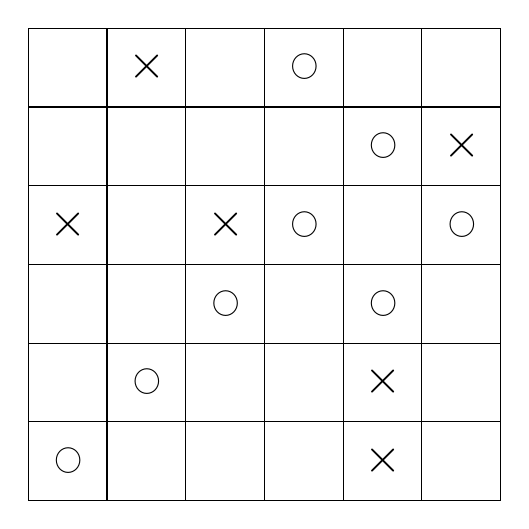
\begin{tikzpicture}
					\draw[step=1cm,color=black] (0,0) grid (6,6);					
					\matrix[matrix of nodes,
					inner sep=0pt,
					anchor=south west,
					nodes={inner sep=0pt,text width=1cm,align=center,minimum height=1cm, color=black}]								{
						 & $\bigtimes$ &  & $\bigcirc$ &  & \\
						 &  &  &  & $\bigcirc$ & $\bigtimes$\\
						$\bigtimes$ &  & $\bigtimes$ & $\bigcirc$ &  & $\bigcirc$\\
						 &  & $\bigcirc$ &  & $\bigcirc$ & \\
						 & $\bigcirc$ &  &  & $\bigtimes$ & \\
						$\bigcirc$ &  &  &  & $\bigtimes$ & \\
					};
				\end{tikzpicture}
%max coins grid
				\bigskip
				\\ Grid of max coins: \textit{(Note: '\textbf{--}' denotes large negative number.)} \\
				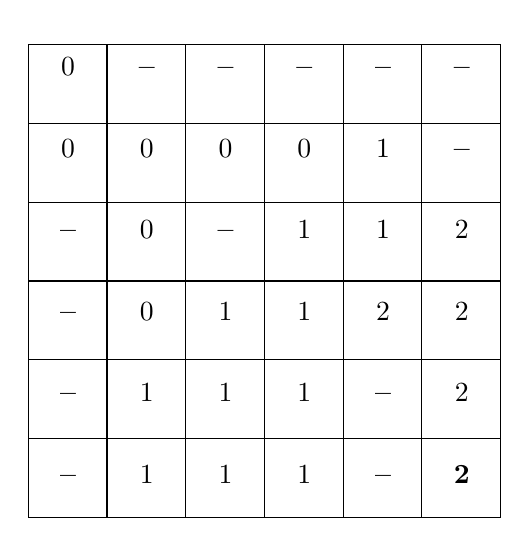
\begin{tikzpicture}
					\draw[step=1cm,color=black] (0,0) grid (6,6);					
						\matrix[matrix of nodes,
						inner sep=0pt,
						anchor=south west,
						nodes={inner sep=0pt,text width=1cm,align=center,minimum height=1cm, color=black}]								{
							0 & \textbf{--} & \textbf{--} & \textbf{--} & \textbf{--} & \textbf{--} \\
							0 & 0 & 0 & 0 & 1 & \textbf{--} \\
							\textbf{--} & 0 & \textbf{--} & 1 & 1 & 2 \\
							\textbf{--} & 0 & 1 & 1 & 2 & 2 \\
							\textbf{--} & 1 & 1 & 1 & \textbf{--} & 2 \\
							\textbf{--} & 1 & 1 & 1 & \textbf{--} & \textbf{2} \\
						};
				\end{tikzpicture}
%path grid				
				\bigskip
				\\ Grid of path: \textit{(Note: multiple optimal paths can be taken.)} \\
				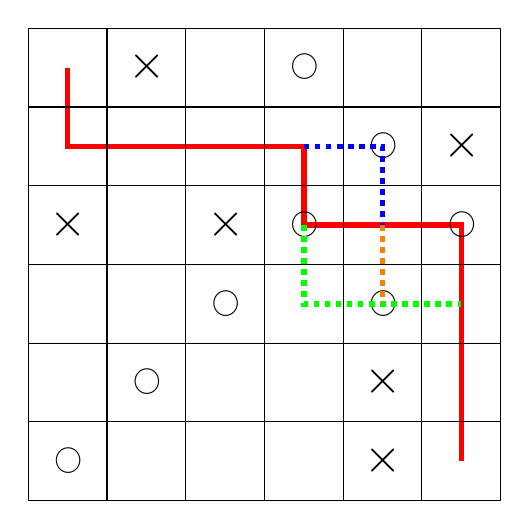
\begin{tikzpicture}
					\draw[line width=2pt, color=red] (5.5,0.5) -- (5.5, 3.5) --  (3.5,3.5) -- (3.5,4.5) -- (.5, 4.5) -- (.5,5.5);
					\draw[step=1cm,color=black] (0,0) grid (6,6);					
						\matrix[matrix of nodes,
						inner sep=0pt,
						anchor=south west,
						nodes={inner sep=0pt,text width=1cm,align=center,minimum height=1cm, color=black}]								{
							 & $\bigtimes$ &  & $\bigcirc$ &  & \\
							 &  &  &  & $\bigcirc$ & $\bigtimes$\\
							$\bigtimes$ &  & $\bigtimes$ & $\bigcirc$ &  & $\bigcirc$\\
							 &  & $\bigcirc$ &  & $\bigcirc$ & \\
							 & $\bigcirc$ &  &  & $\bigtimes$ & \\
							$\bigcirc$ &  &  &  & $\bigtimes$ & \\
						};
					\draw[dotted, line width=2pt, color=blue](3.5,4.5) -- (4.5,4.5) -- (4.5,3.5);
					\draw[dotted, line width=2pt, color=green](3.5,3.5) -- (3.5,2.5) -- (4.5,2.5) -- (5.5,2.5);
					\draw[dotted, line width=2pt, color=orange](4.5,3.5) -- (4.5,2.5);
				\end{tikzpicture}
		\end{enumerate}

\end{enumerate}

\end{document}
